\chapter{Computational Model} \label{model}

\newcommand{\numcategories}[0]{$n_{cat}$ }
\newcommand{\numsubcategories}[0]{$cat$ }
\newcommand{\numsensors}[0]{$N_S$ }
\newcommand{\numstakeholders}[0]{$N_{DC}$ }
\newcommand{\numcontexts}[0]{$N_C$ }
\newcommand{\numquestions}[0]{$n_{dr}$ } 
\newcommand{\numsubfeatures}[0]{$n_{sf}$ } 



\section{Introduction}
A data request is a request to users to trade their mobile sensor data. The aim is to create a computational model that is able to assign personalized rewards to each data request for every user.
Each user is associated with a privacy intrusion profile. The model uses the user profiles to assign each data request a maximum achievable reward. The model attempts to identify the data requests where users might not be inclined to share mobile sensor data. These data requests are assigned a higher maximum obtainable reward. Similarly, the data requests where the users would want to share more mobile sensor data
are assigned a lower maximum obtainable reward. This permits to see whether incentives do indeed make a difference in mobile sensor
data sharing. The model aims to identify the amount of data each user would share for a data request and assign maximum obtainable rewards accordingly.

\section{Model}

\begin{figure}[ht!]
\centering
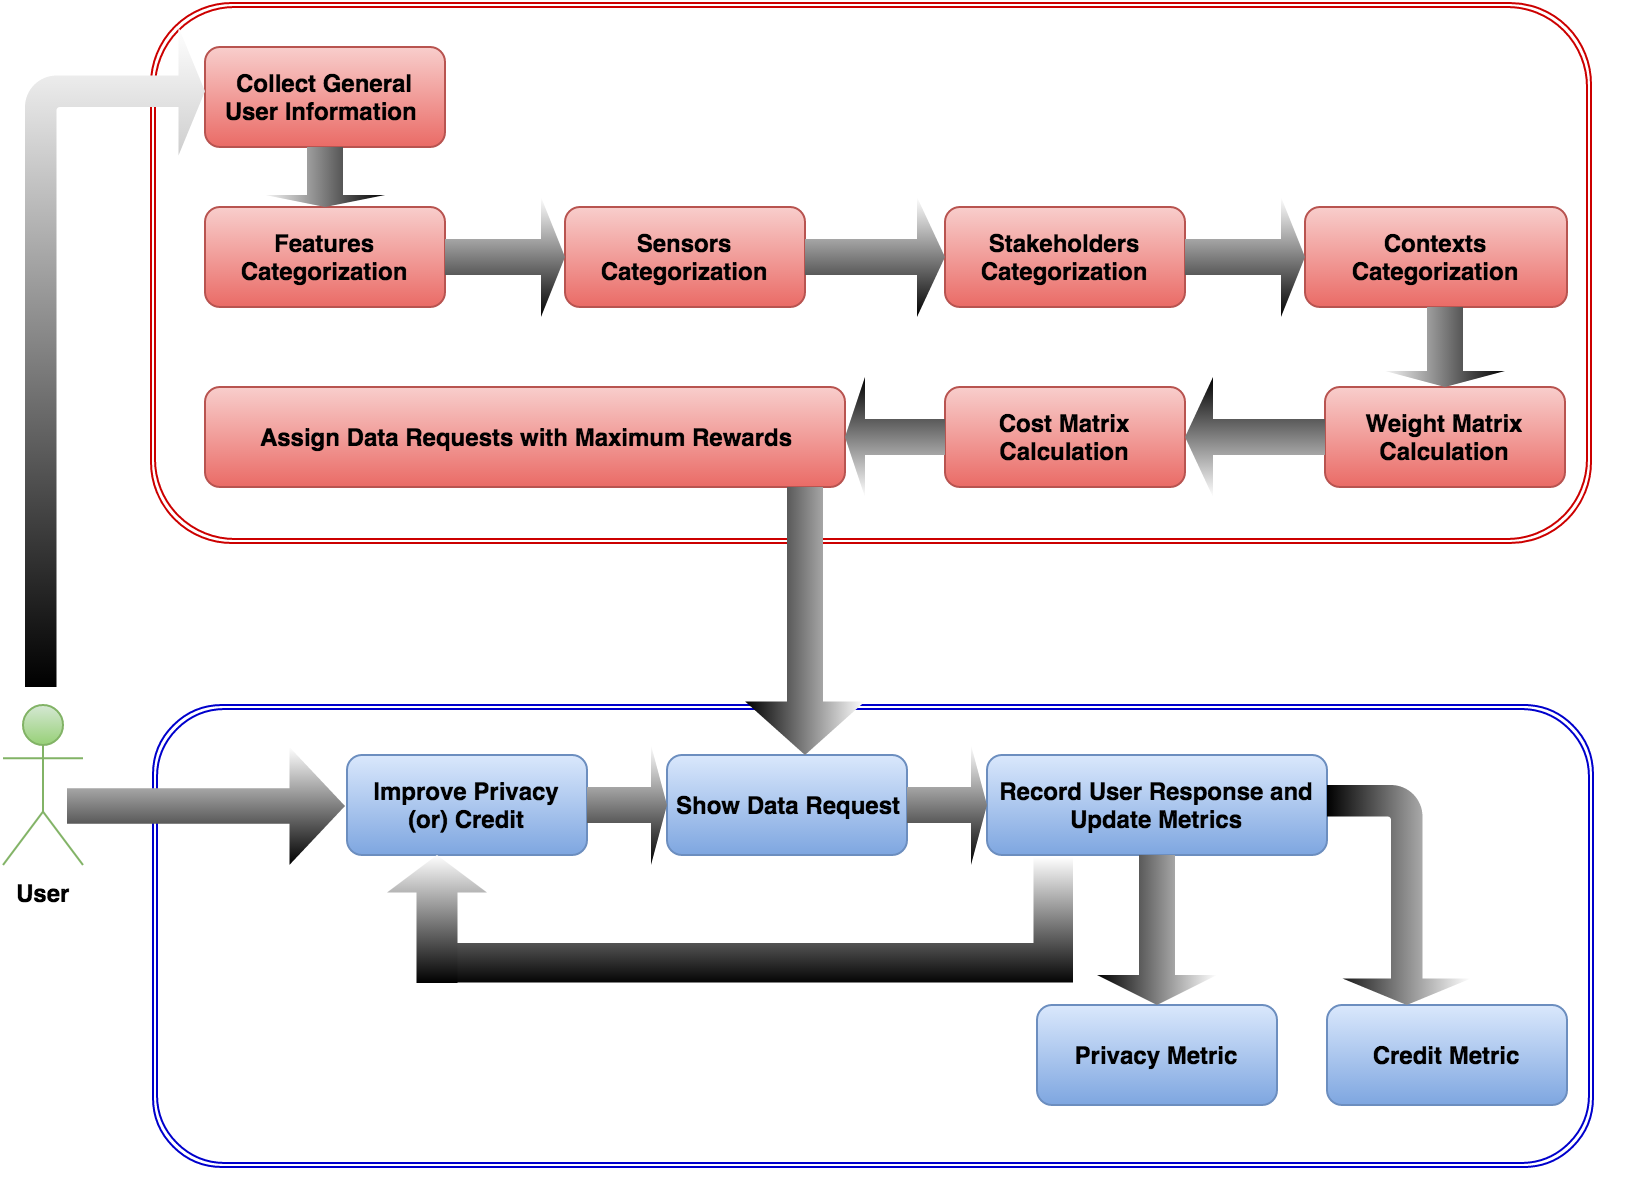
\includegraphics[width=\textwidth,keepaspectratio	]{./images/model_building_blocks}
\caption{Computational model flow chart \label{model_blocks}}
\end{figure}

The sections below explain the various building blocks of the computational model. Figure \ref{model_blocks}
provides an overview of the flow of the model.

\subsection{Collecting User Information}
To begin with, user information is collected. The information collected consists of but is not limited to :

\begin{itemize}
\item Gender
\item Year of birth
\item Country
\item Education Level
\item Occupation
\item Frequency of mobile phone use per day
\item List of different mobile applications present on the users phones
\end{itemize}

%Collecting this information is crucial to the data analysis that is conducted in the later stages.
\subsection{Categorization of the Features} \label{catfeatures}

Features are the aspects that govern the data sharing decision. A feature can be one of the following:
\begin{itemize}
\item \textbf{Sensors} : They consist of the data obtained from sensors in the mobile phone that users can trade for a data request
\item \textbf{Stakeholders} : They consist of any entity that requests users for mobile sensor data
\item \textbf{Contexts} : They consist of the purpose for which a stakeholder would like to obtain the user's mobile sensor data
\end{itemize}

Features are placed in categories according to how privacy intrusive they are. Features are the three dimensions that form a data request. A data request is defined as a stakeholder asking users to share their mobile sensor data for a particular context. Users are asked to categorize the features into one of the five categories:

\begin{enumerate}
\item Very low privacy intrusion
\item Low privacy intrusion
\item Medium privacy intrusion
\item High privacy intrusion
\item Very high privacy intrusion
\end{enumerate}

Categories are linearly scaled and equally spaced. As indicated by the numbers on the left of the categories, these range from 1 to 5 and users can place each of the features in a category according to their perceived intrusion level. Category 1 represents that the feature does not at all contribute to the data sharing decision. Similarly, category 5 represents that the feature contributes to the maximum possible for the user's data sharing decision. It represents that users are reluctant to give away their sensor data for this feature. More than one feature can be placed in the same category.

Let the variable \numcategories represent the number of categories, which here are five. Additionally, let the category assigned to the sensors be represented by the variable $a$, the category assigned to the stakeholders be represented by the variable $b$ and the category assigned to the contexts be represented by the variable $c$.

Once the sensors, stakeholders and the contexts are categorized into the respective categories reflecting the importance of each of the features in the data sharing decision, each feature is assigned a weight. Let the respective weights of sensors, stakeholders and contexts be represented by the variables, $w_{a}$, $w_{b}$ and $w_{c}$ and calculated as follows:

\begin{equation}
   w_{a} = \frac{a}{a+b+c} 
\end{equation}
\begin{equation}
   w_{b} = \frac{b}{a+b+c}   
\end{equation}
\begin{equation}
   w_{c} = \frac{c}{a+b+c}   
\end{equation}

\subsection{Categorization of the Sub-Features}
After the feature categorization and their weights computed as above, sub-features categorization takes place. A sub-feature
is defined as a type of a feature. In other words, sub-features are the different types of features that appear during data request to the user. The following are examples of sub-features for each feature :

\begin{itemize}
\item Sensors : 
\begin{itemize}
\item Accelerometer
\item  Battery
\item Gyroscope
\end{itemize} 
\item Stakeholders : 
\begin{itemize}
\item Corporation
\item  Government
\item Educational institution
\end{itemize}
\item Contexts :
\begin{itemize}
\item Education
\item Navigation
\item Gaming
\end{itemize}
\end{itemize}

\begin{figure}[ht!]
\centering
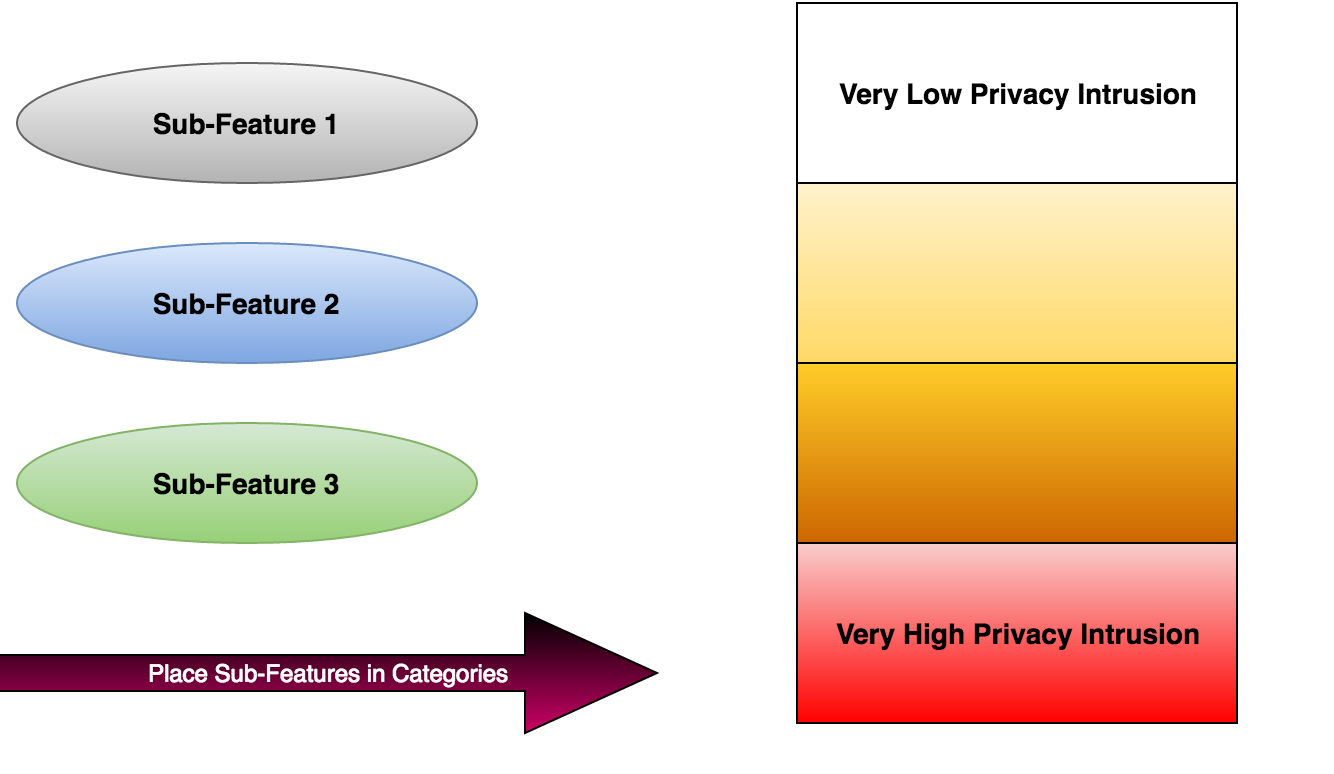
\includegraphics[width=\textwidth,keepaspectratio]{./images/categorize_sub}
\caption{Categorizing sub-features according to the perceived intrusion level \label{categorize_sub}}
\end{figure}

Each of the above are different kinds or sub-features of the respective features. 
For each of the available features, the respective sub-features need to be in turn categorized as mentioned in Section \ref{catfeatures}. The categories are also the same as mentioned in Section \ref{catfeatures}. Let \numsubfeatures be the number of sub-features each feature has. It is assumed that each feature has the same number of sub-features.

As seen in the conceptual diagram which is shown in Figure \ref{categorize_sub}, users place each of the sub-features available for every feature in the given categories.

Let every sub-feature be represented by unique indices within its feature. For example, in the list of sub features provided above, accelerometer is the first sub-feature of sensors, corporation is the first sub-feature of stakeholders and education is the first sub-feature of contexts. For each of the sub-features of sensors, categories they are placed in by users is represented by $a_{i}$ and $i$ is the index
of the sub-feature. Similarly, categories assigned to sub features of feature stakeholders and contexts respectively are represented by $b_{j}$ and $c_{k}$, where $j$ and $k$ are the identifiers of the sub-features categorized.

\subsection{Weight Matrix Calculation}
Each data request consists of the three above mentioned features in them. Each of the features have \numsubfeatures sub-features that can appear in turns in a data request assuming that each feature has the same number of sub-features. The total number of possible data requests are $n_{dr} =  n_{sf}^3$.

Let $W$  be a matrix with three dimensions $n_{sf}$ x $n_{sf}$ x $n_{sf}$. We call this the weight matrix.
Each cell of $W$, that is $W_{i,j,k}$ represents a data request which involves the sensors sub-feature with identifier $i$, stakeholders sub-feature with identifier $j$,
and the contexts sub-feature with identifier $k$. That is, each cell of $W$ represents the weight of a data request to the user. The aim of the weight matrix is to use the information collected from the user categorizations, to assign weights to each data request. Intuitively, the process examines the
data requests where the user is least likely to trade data and assigns higher weights to those data requests. This process is seen in
Section \ref{analysis_model} with examples. As mentioned before, each cell of the matrix $W$ represents the weight of a data request with a unique sensor sub-feature $i$, stakeholder sub-feature $j$ and context sub-feature $k$. To calculate the weight of a data request :

\begin{equation}
W_{i,j,k} = (a*a_{i}) + (b*b_{j}) + (c*c_{k})
\end{equation}

Applying this formula for every possible $i$, $j$ and $k$ gives the weight matrix $W$.

\subsection{Cost Matrix Calculation}

The aim is now to assign maximum obtainable rewards to each data request. This reward is the maximum credit users can receive for a particular data request. Let $C$ be the cost matrix with the three dimensions $n_{sf}$ x $n_{sf}$ x $n_{sf}$.
Let it be assumed to have a budget of $B$ for a day, where
$B$ can be in an actual currency or any form of virtual credits. In this chapter, the unit for budget is credits. Each cell of the cost matrix represents the amount of rewards allocated for a particular data request for one day.
To begin with, we calculate the sum of all the cells of the weight matrix $W$:

\begin{equation}
s_{W} = \sum\limits_{i=1}^{n_{sf}} \sum\limits_{j=1}^{n_{sf}} \sum\limits_{k=1}^{n_{sf}} W_{i,j,k}
\end{equation}

Where the function $s_{W}$ gives the sum of a matrix, in this case the weight matrix.
Let $C_{i,j,k}$ represent the credit allocated for the data request which involves the sensor's sub-feature with identifier $i$, stakeholder's sub-feature with identifier $j$, and the context's sub-feature with identifier $k$. To calculate one cell of the cost matrix :

\begin{equation}
C_{i,j,k} = \frac{W_{i,j,k} * b}{s_{W}}
\end{equation}

Repeating the above for every cell of $C$, the entire cost matrix is calculated. Now, all the maximum obtainable rewards are allocated per day for every data request.

\subsection{Cost and Privacy Metrics} \label{o}
Every data request is assigned a reward. This is the maximum reward that a user can obtain for that data request.
The cost metric is the amount of rewards the user obtains by trading sensor data for each data request. Similarly, the privacy metric is the amount of privacy percentage the user obtains while trading data for data requests. It quantifies the amount of data the user has refused to share hence implying privacy. The cost and privacy metrics are inversely proportional to each other, in the sense that when the cost metric increases the privacy metric decreases and vice versa.

In each data request, one chooses how much data is to be shared, from the maximum amount of data to no data at all. The possible responses to a data request are called options. Each option corresponds to a summarization level explained in Section \ref{summa}. The reward assignment to each option is linearly scaled according
to the reward assigned to each data request. Let us assume there are options for a data request ranging from $1$ to $m$ (numeric options), where $1$ corresponds to the option where the users give all their data for a request and $m$ to where the users choose not to give any data for a request. Therefore there are a total of $m$ options for every data request. Each option in a data request has the following:

\begin{itemize}
\item The amount of change in the cost metric if this particular option for a data request is chosen
\item The amount of change in the privacy metric if this particular option for a data request is chosen
\end{itemize}

While assigning rewards to data requests there are two scenarios to consider:

\begin{itemize}
\item Assigning option rewards without a participation reward. Users are not rewarded for responding to data requests
\item Assigning option rewards inclusive of a participation reward. Users are rewarded for responding to data requests irrespective of the option chosen
\end{itemize}

Let us examine the first scenario. Let the option rewards be calculated for the data request with sensor sub-feature $i$, stakeholder sub-feature $j$ and
context sub-feature $k$. The assigned reward for any option numbered $h$ of this data request is calculated as follows:

\begin{equation}
r_{h} =  \frac{C_{i,j,k}*(m-h)}{m-1}
\end{equation}
%This concept can be implemented to ensure user participation in the experiment.
Applying this formula by replacing $h$ by the option numbers from $1$ to $m$ gives the reward that the user can receive for each option.
Similarly, if a participation reward is assigned to each option, it means that even tough the user does not share data, they still
receive rewards for answering the data request. Let $x$ be a fraction of the total budget $B$ that is dedicated for user participation. Using geometric progression with $a=1$ and $z=\sqrt[(m-1)]{x}$ , we can calculate the fraction $f_{h}$ of the maximum reward obtainable from a data request an option numbered $h$ gets:

\begin{equation}
f_{h} = a * z^{h-1}
\end{equation}

The fraction of the rewards an option $h$ is assigned is calculated. To obtain the rewards $r_{h}$ of an option $h$ for a data request with sensor sub-feature $i$, stakeholder sub-feature $j$ and
context sub-feature $k$ :

\begin{equation}
r_{h} = f_{h} * C_{i,j,k}
\end{equation}
This assigns rewards to each option, taking into consideration participation rewards that the user gets even if data is not shared for that data request.

Privacy percentage $p_{h}$ is linearly scaled between the first to the $m^{th}$ option between $0$ and $1$ as follows:
\begin{equation}
p_{h} = \frac{(h-1)}{m-1}
\end{equation}

The total cost and privacy is the sum and arithmetic average of all the rewards and privacy respectively, obtained from every answered data request. If a data request is unanswered, a maximum privacy of 1 and minimum cost of 0 credit is assumed.


\subsection{Improving the Metrics}
%(Less like experiment)
%Before users answer a data request, it is useful to know where the user interest lies in. Would the user like to improve
%the privacy metric, or would the user would like to increase the credit revenue. In addition, if we know what the user is looking to improve, we can retrieve the data request that has the possibility to improve that particular metric the most.
%For example if the user wishes to improve his privacy further, we look at the questions where the user has given the most amount of data. We then put forth this question to answer, which indicating all the options that can improve the privacy. Similarly, if the user chooses to obtain more credit, the question where the user has given least amount of data is retrieved. Options that can improve the user credit are also indicated.
Users can choose to improve the privacy or cost metric. If the user chooses to gain more rewards (improve the cost metric), the data request where maximum rewards can be obtained is fetched. Otherwise, if users want to improve their privacy the data request which can maximize the privacy is obtained. Additionally, each option of a data request indicates the change in the metrics that take place if that option is chosen.

\subsection{Summarization of Collected Data} \label{summa}
Each data request has the possibility to have $m$ number of options the user can choose for every data request. These options range from $1$, which indicates that users would like to give all their data, to option number $m$, which indicates that users do not want to give any data to this request.

Summarization is a privacy algorithm that modifies the quality of data to provide less information than in its original form \cite{pournaras2016self}. A higher summarization level gives data with lower quality. A lower summarization level gives data with higher quality. In this model, sensor data is collected for a period of $d$ hours every $y$ seconds for every data request. If the data is summarized, according to the summarization level (option) chosen, the data is collected either every $y$ seconds or less.

Data is collected for a period of $d$ hours, and at the end of this period it is summarized according to the option chosen for the data request. Summarization can
be linearly assigned to each option.
The highest privacy option $m$ corresponds to the highest summarization level. The first option corresponds to the lowest summarization level. An example of assigning the summarization level $l_{h}$ for an option h for a data request has the possibility of the following :
\begin{equation}
l_{h} = y*h \text{ where } h \neq m
\end{equation}

This gives the frequency of sensor data collection for every option of a data request.

\section{Analysis of the Model} \label{analysis_model}
In this section presents three different examples in order to witness some properties of the weight and cost matrices.

\subsection{Setup}
In the following examples, the following features and sub-feature are considered:

\begin{enumerate}
    \item Sensors
    \begin{enumerate}
    \item Accelerometer 
    \item Noise 
    \item Location 
   \end{enumerate}
    \item Stakeholders 
    \begin{enumerate}
    \item Corporation 
    \item Government 
    \item Educational institution 
   \end{enumerate}
   \item Contexts
    \begin{enumerate}
    \item Navigation 
    \item Environment 
    \item Social Media 
   \end{enumerate}
 \end{enumerate}
 
Number indications to the left of the sub-features are the corresponding unique indices. This uniquely identifies a sub-feature within a feature. There are in total $num_{sf}=3$ sub-features for each feature.
Each user receives a number of $num_{sf}^3=27$ data requests in total. The number of categories available to categorize is $n_{cat}=5$ as explained in Section \ref{catfeatures}. Additionally, the budget is $B=100$ CHF per day. 
The input to the model are the user choices during the categorization of the features and sub-features.

\subsection{Examples}

To make referencing easier to the graphs, instead of sub-feature names, numeric indices are used. From now each feature and sub-feature is referred to by its index such as feature 1 for sensors and sub-feature 2 of feature 1 for the noise sensor. The tuple (a,b,c) represents a data request with:
\begin{enumerate}
    \item a - Sensor's sub-feature a
    \item b - Stakeholder's sub-feature b
    \item c - Context's sub-feature c
   \end{enumerate}
where a, b and c are all numbers from one to three. 


If features and sub-features all have the same categories assigned by users respectively, then all data requests should be assigned equal weights and rewards. In example 1, users choose categories for the features and sub-features as shown in Table \ref{tab:scenario11}. From this input, the formulation of the weight matrix is shown in Figure \ref{weight11}, and the cost matrix is shown in Figure \ref{cost11}.
For each data request indicated as a tuple (sensors, stakeholders, contexts) in the x-axis of Figures \ref{weight11} and \ref{cost11}, all have identical weights and rewards. This is due to the fact that the users find all the features and sub-features equally intrusive so all the data requests are weighed equally.

\begin{table}[h!]
  \centering
  \caption{Categorization for example 1}
  \label{tab:scenario11}
  \begin{tabular}{cccc}
    \toprule
    Feature & Sub-Feature 1 & Sub-Feature 2 & Sub-Feature 3\\
    \midrule
    Sensors & Accelerometer & Noise & Location\\
     1 & 3 & 3 & 3\\ \hhline{====}
     Stakeholders & Corporation & Government & Educational Institution\\
     1 & 3 & 3 & 3\\ \hhline{====}
     Contexts & Navigation & Environment & Social Media\\
     1 & 3 & 3 & 3\\ 
    \bottomrule
  \end{tabular}
\end{table}
 
\begin{figure}[htp]
  \subtop[Weight matrix example 1\label{weight11}]{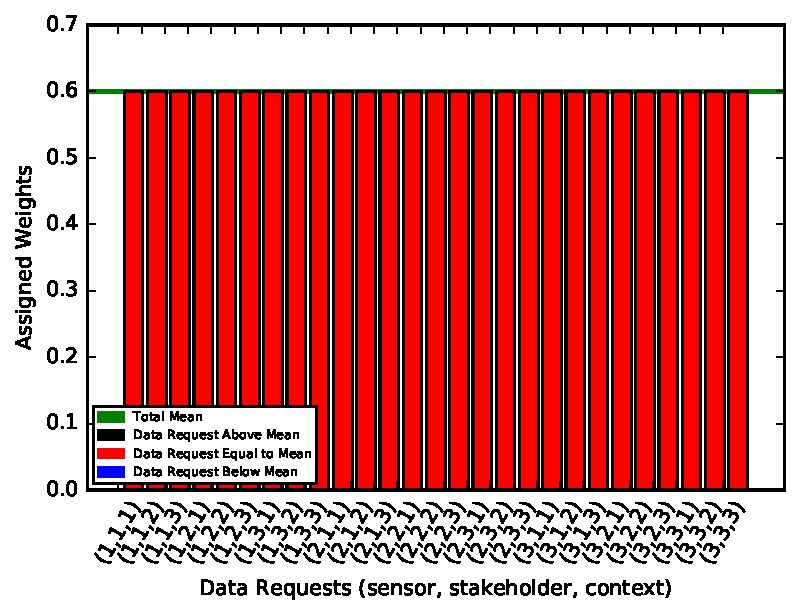
\includegraphics[width=0.5\linewidth]{./images/weight_1_1}}\hspace{1em}
  \subtop[Cost matrix example 1 \label{cost11}]{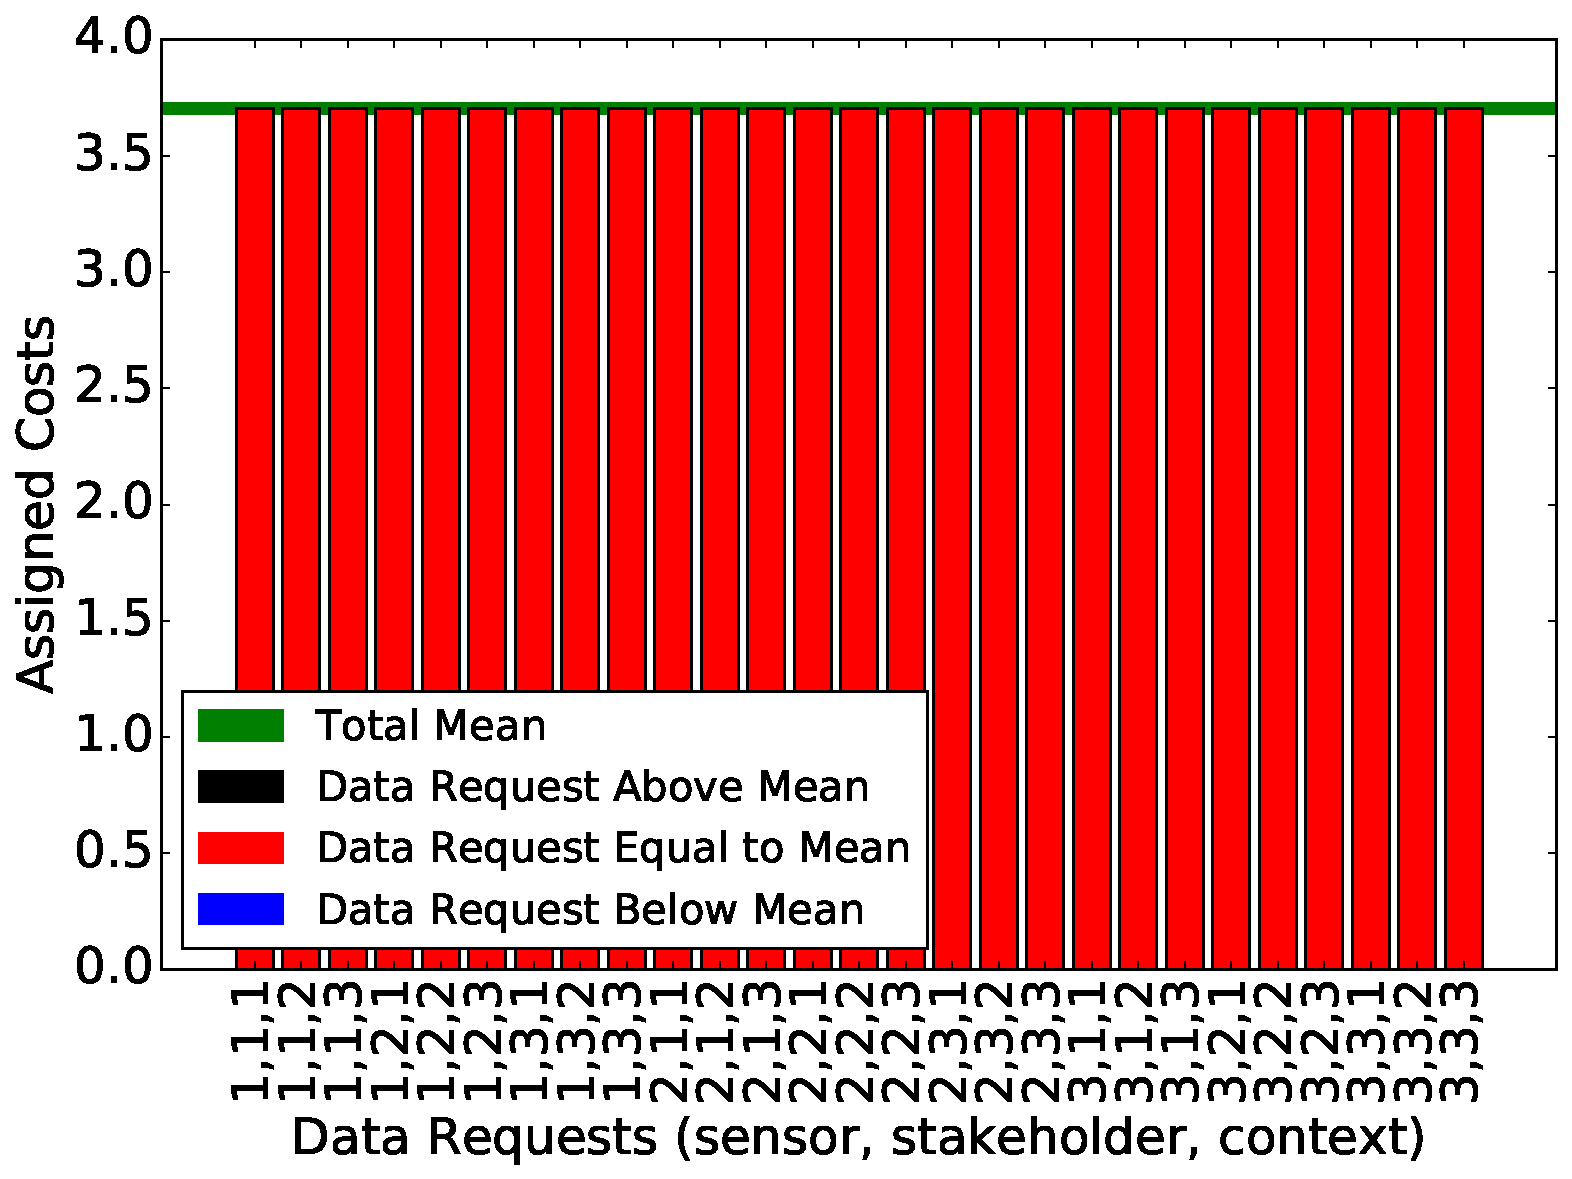
\includegraphics[width=0.5\linewidth]{./images/cost_1_1}}\newline
   \subtop[Weight matrix example 2\label{weight3}]{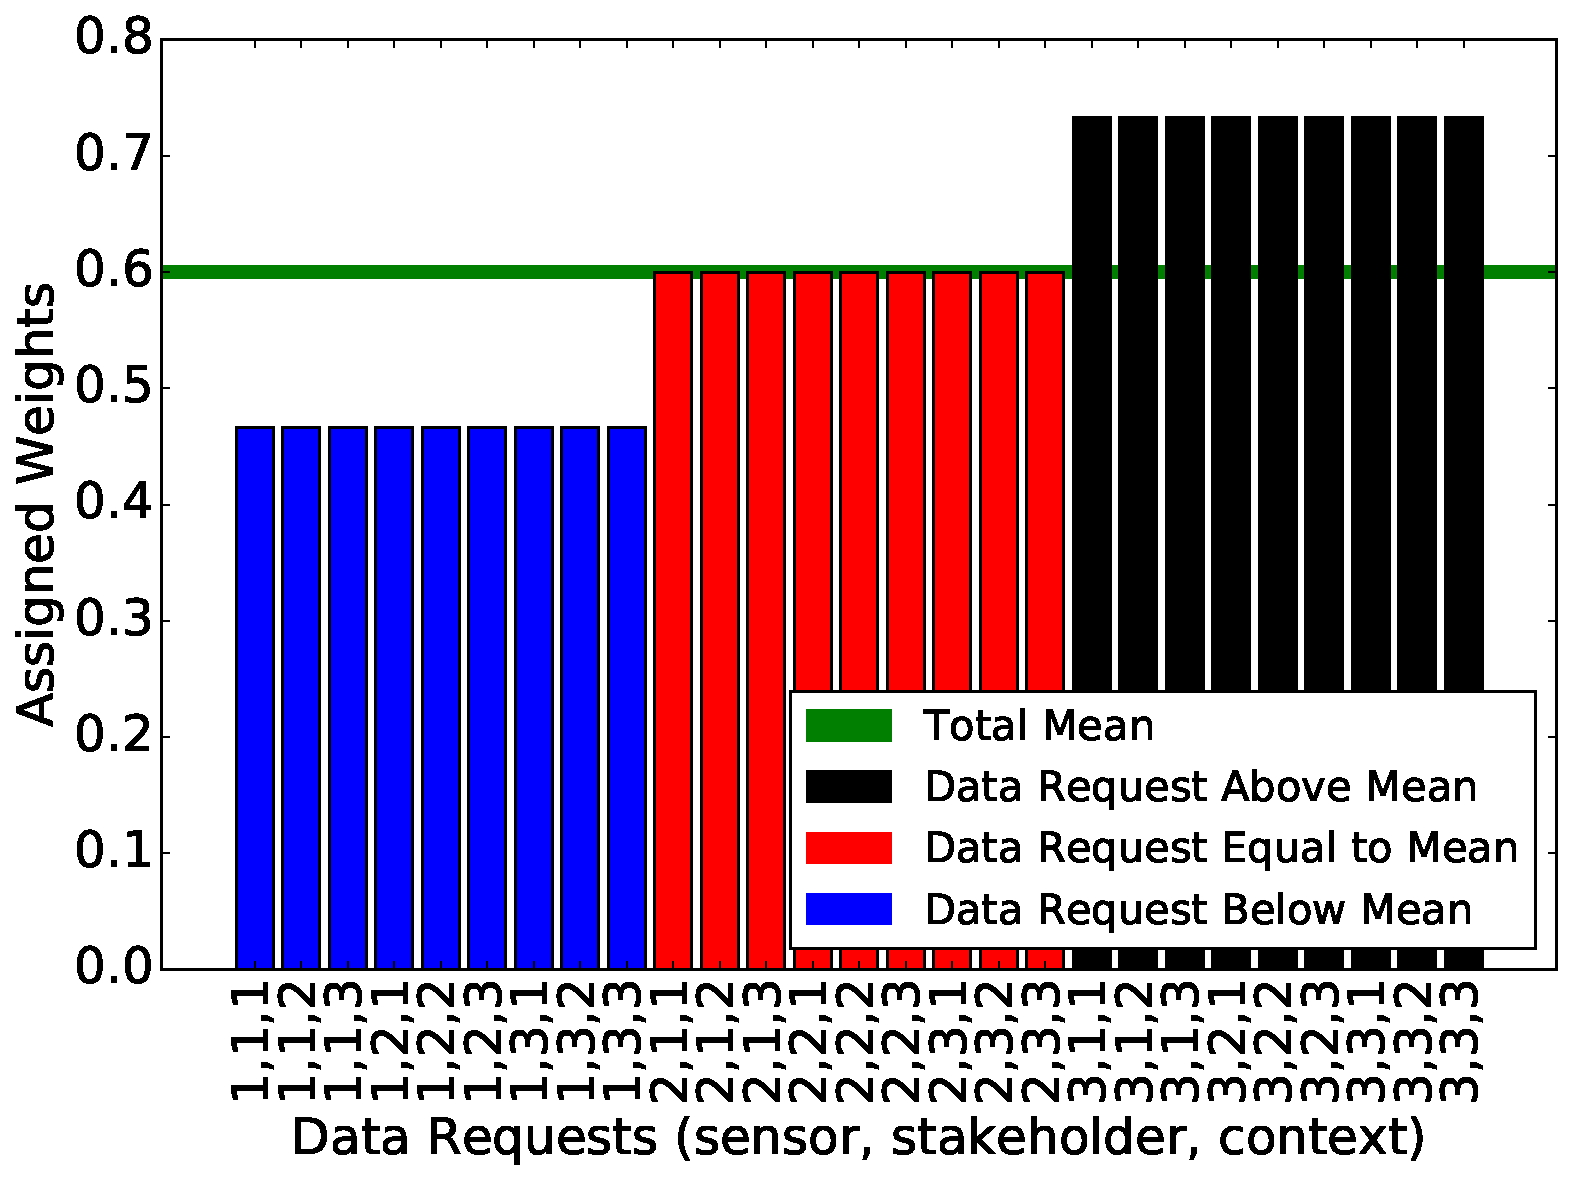
\includegraphics[width=0.5\linewidth]{./images/weight_3}}\hspace{1em}
  \subtop[Cost matrix example 2\label{cost3}]{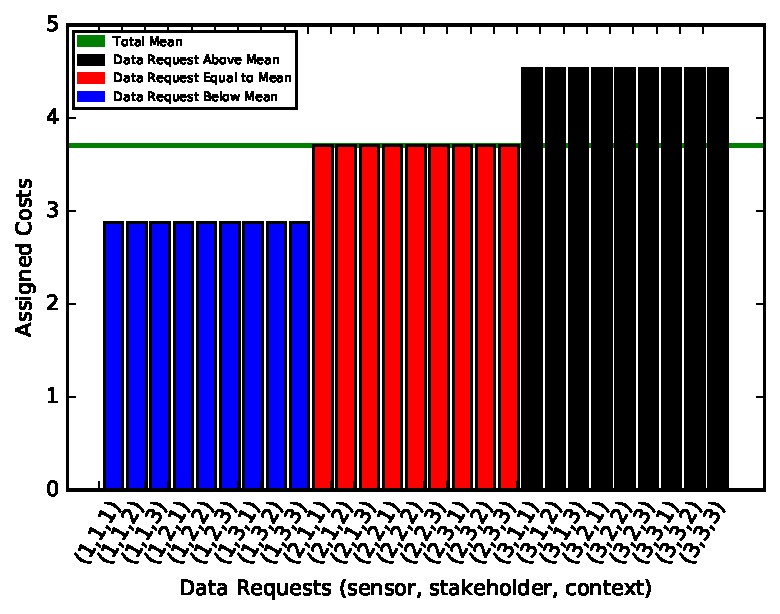
\includegraphics[width=0.5\linewidth]{./images/cost_3}}\newline
  \subtop[Weight matrix example 3\label{weight4}]{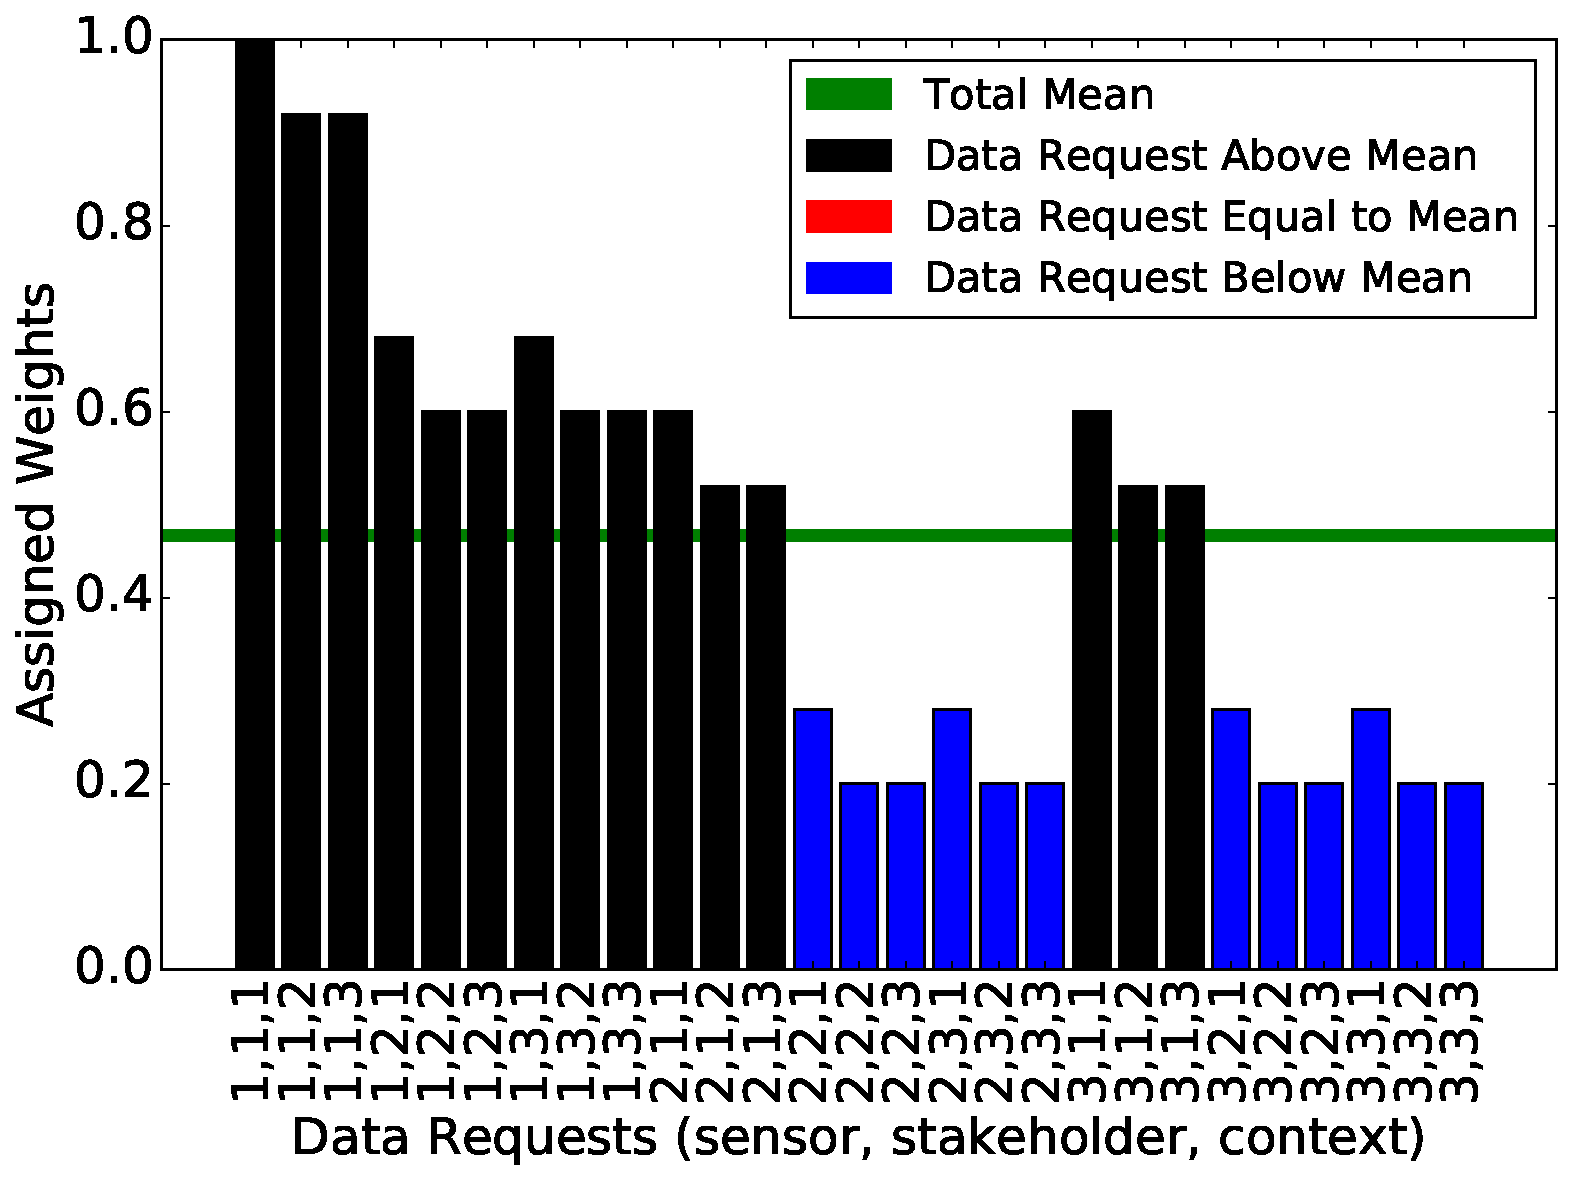
\includegraphics[width=0.5\linewidth]{./images/weight_4}}\hspace{1em}
\subtop[Cost matrix example 3\label{cost4}]{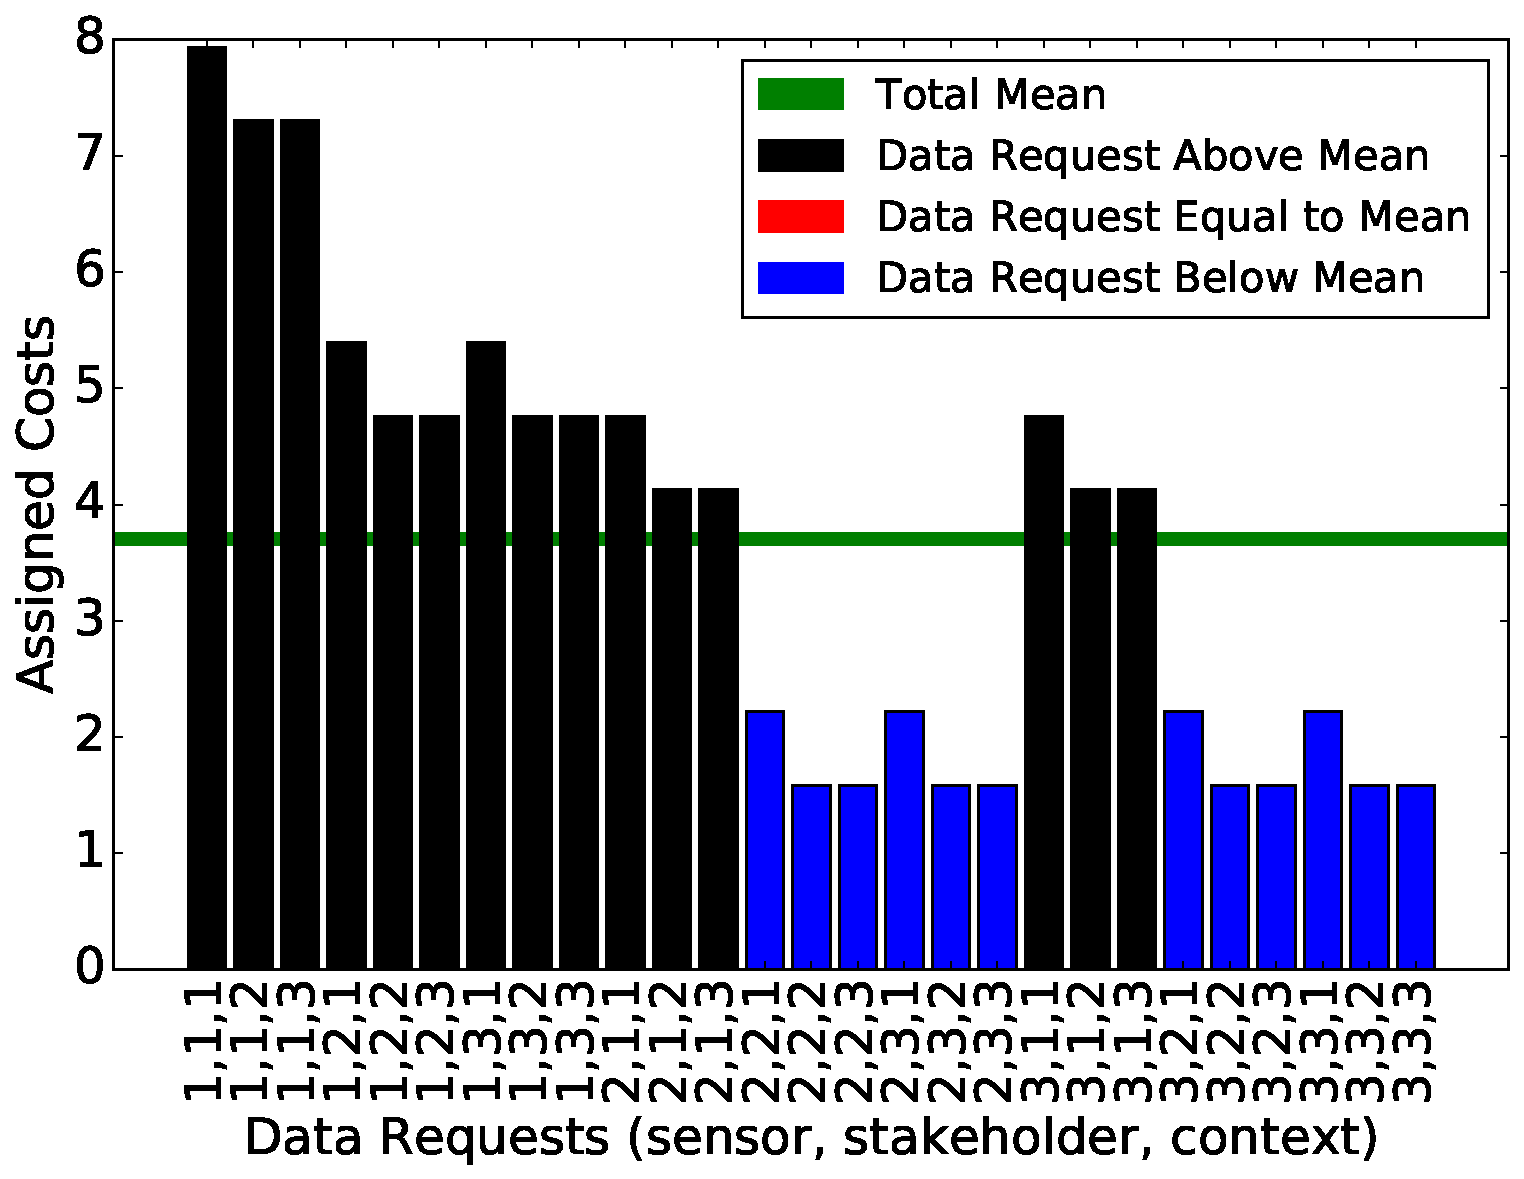
\includegraphics[width=0.5\linewidth]{./images/cost_4}}
  \caption{Values assigned to matrices}
  \label{fig:scenatio11}
\end{figure}

%\begin{figure}[ht!]
%\centering
%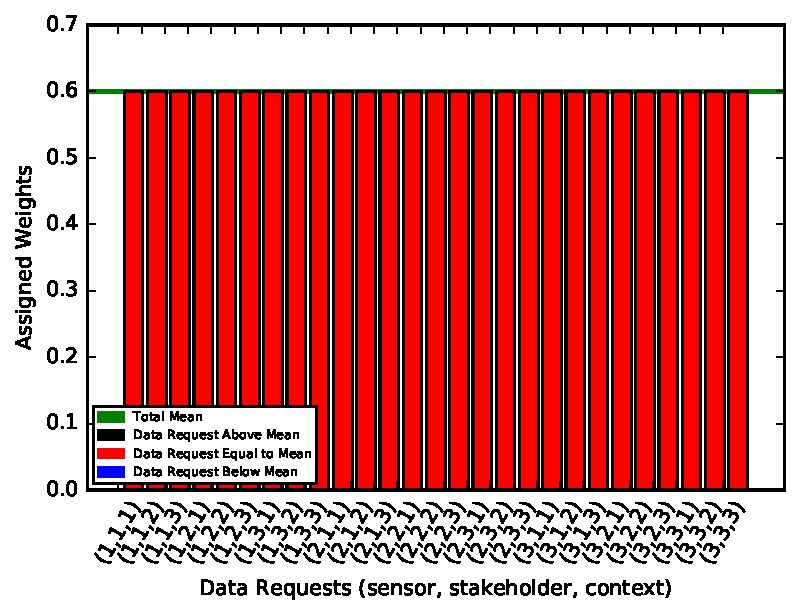
\includegraphics[width=\textwidth,keepaspectratio]{./images/weight_1_1}
%\caption{Values of the Weight Matrix \label{weight11}}
%\end{figure}
%
%\begin{figure}[ht!]
%\centering
%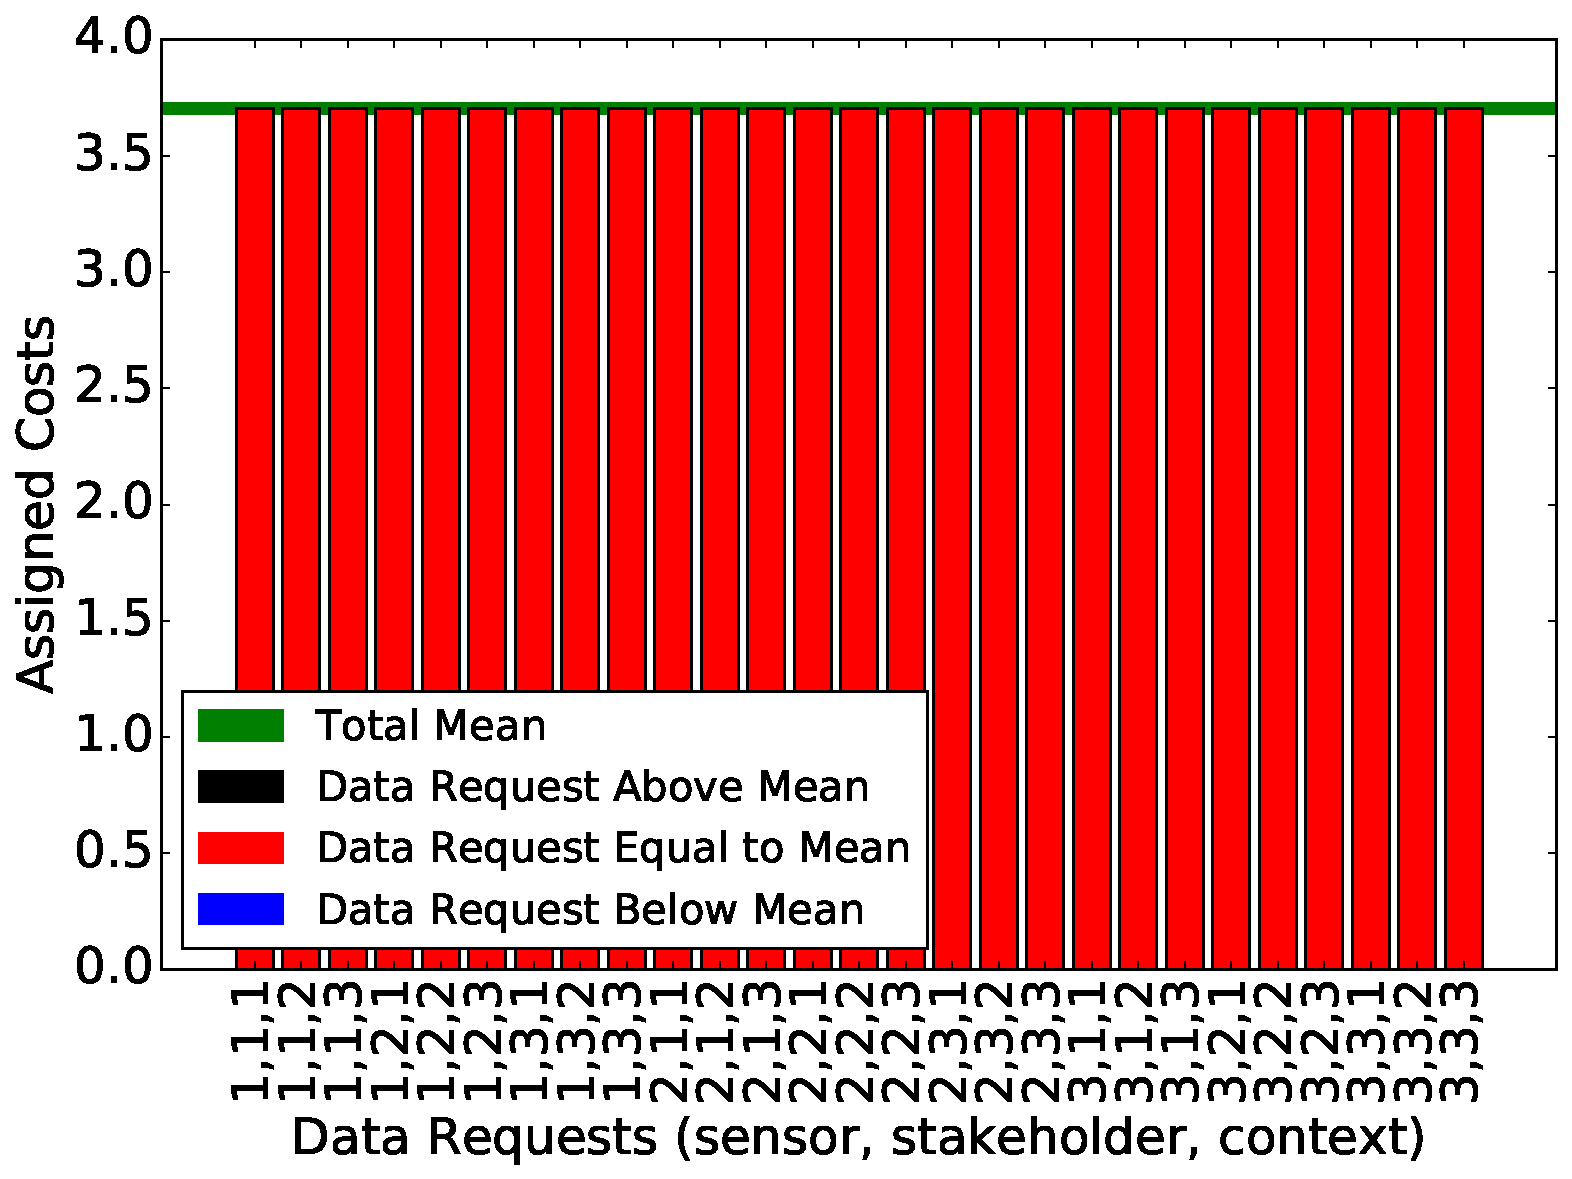
\includegraphics[width=\textwidth,keepaspectratio]{./images/cost_1_1}
%\caption{Values of the Cost Matrix \label{cost11}}
%\end{figure}

If the users perceive features and respective sub-features in an equally intrusive way, then all the
data requests receive the same weight and reward assignments.

Example 2 shows the difference in weight assignments to data requests containing sub-features with higher intrusion levels.
Table \ref{tab:scenario3} indicates the user input. As it is seen, all features have equal categories, and
all sub-features have the categories of 3 with an exception of the sensor sub-features. The sensor sub-features with indices 1,2 and 3 have  categories 1,3 and 5 respectively. This means that requests with sensor sub-feature 1 are assigned a lesser weight in comparison to the other sensor sub-features. 

Similarly, the data requests with sensors sub-feature 2 have a higher weight assigned than sensor sub-feature 1 because of its higher category, but lower than sensor sub-feature 3. Lastly, data requests with sensor sub-feature 3 have the highest weight compared to others, due to the category being 5. The weight and cost matrices are seen in Figures \ref{weight3} and \ref{cost3} respectively.

\begin{table}[h!]
  \centering
  \caption{Categorization for example 2}
  \label{tab:scenario3}
  \begin{tabular}{cccc}
    \toprule
    Feature & Sub-Feature 1 & Sub-Feature 2 & Sub-Feature 3\\
    \midrule
    Sensors & Accelerometer & Noise & Location\\
     3 & 1 & 3 & 5\\ \hhline{====}
     Stakeholders & Corporation & Government & Educational Institution\\
     3 & 3 & 3 & 3\\ \hhline{====}
     Contexts & Navigation & Environment & Social Media\\
     3 & 3 & 3 & 3\\ 
    \bottomrule
  \end{tabular}
\end{table}

%\begin{figure}[htp]
% 
%  \caption{Examining Scenario 2}
%  \label{fig:scenatio3}
%\end{figure}


%\begin{figure}[ht!]
%\centering
%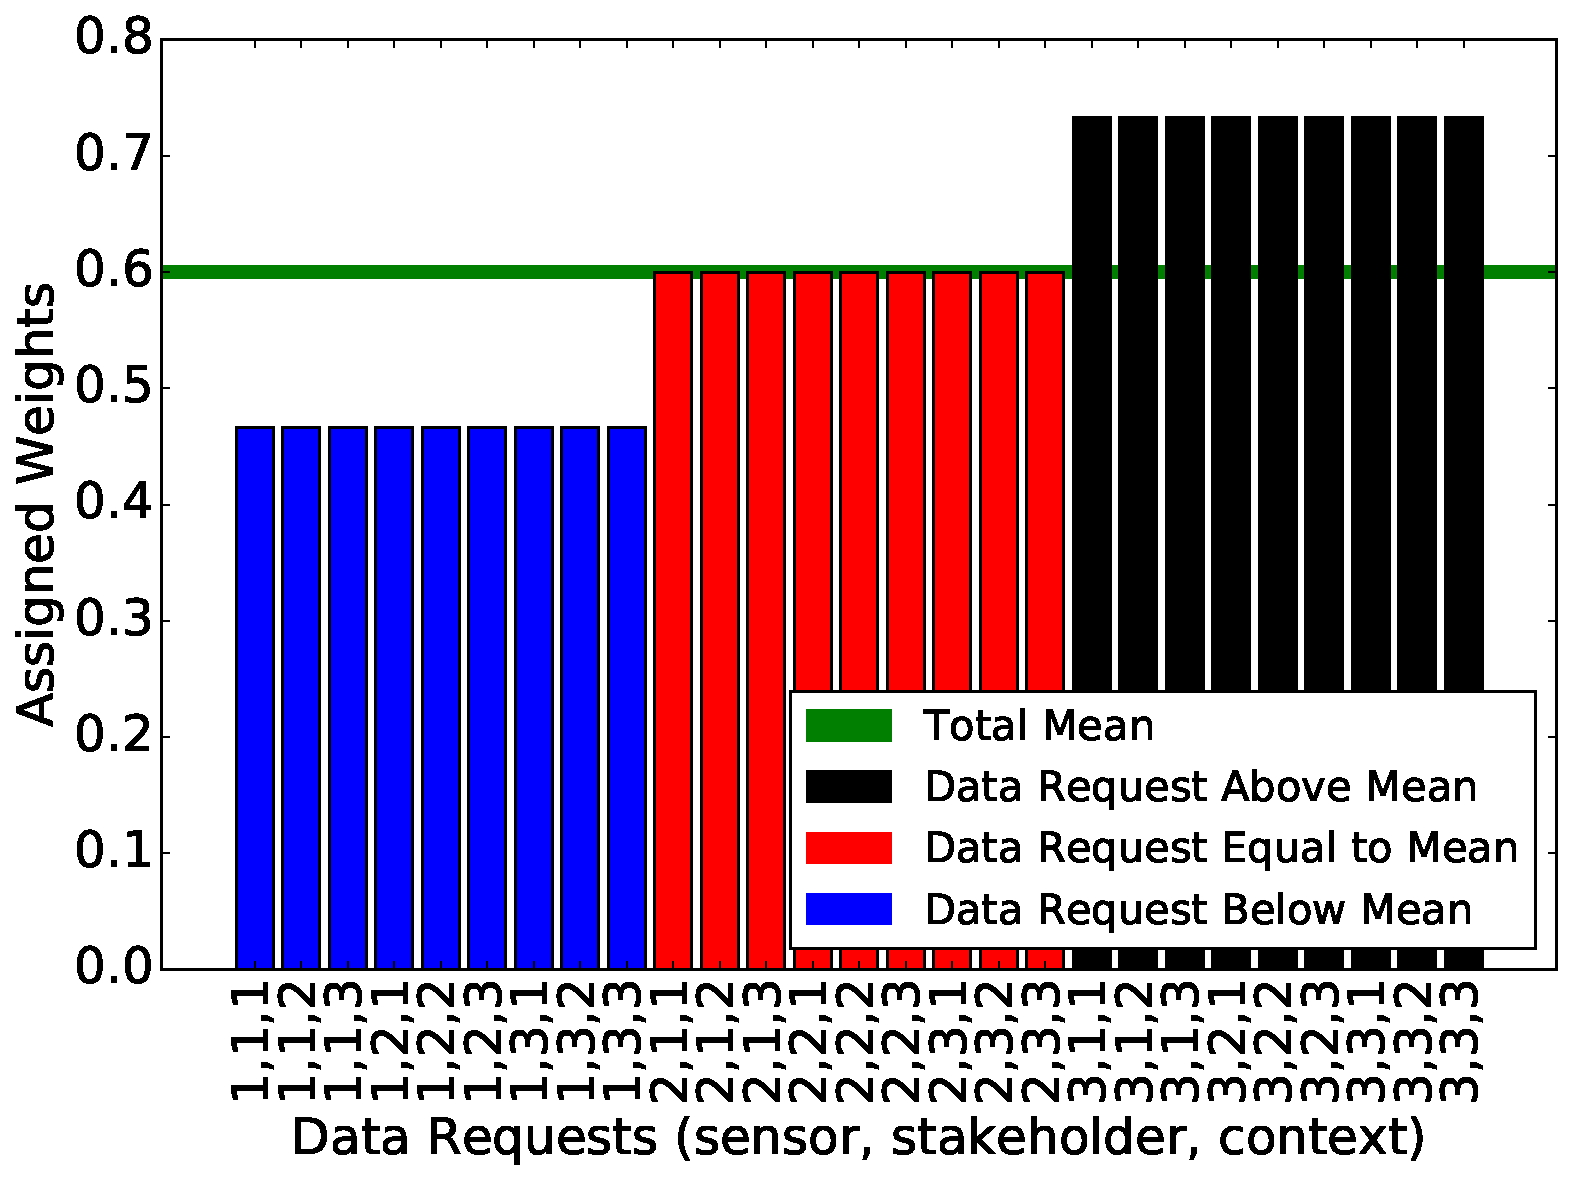
\includegraphics[width=\textwidth,keepaspectratio]{./images/weight_3}
%\caption{Values of the Weight Matrix \label{weight3}}
%\end{figure}
%
%\begin{figure}[ht!]
%\centering
%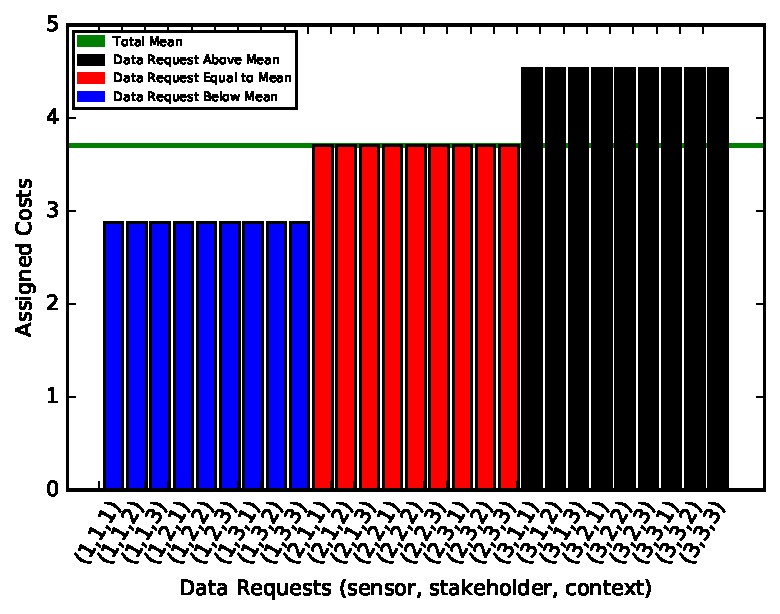
\includegraphics[width=\textwidth,keepaspectratio]{./images/cost_3}
%\caption{Values of the Cost Matrix \label{cost3}}
%\end{figure}


The model assigns a higher weight to data requests with sub-features that users find more intrusive compared to the others.

In example 3, the feature and sub-feature categories are assigned different values, to show how varying their values together affects the assignment of the weight and cost matrix. Table \ref{tab:scenario4} is the user input. All features have different categories assigned from 3 to 5. Additionally, sub-feature 1 of each feature has a category of 5, higher than the other sub-features which are all categorized as 1. The weight and cost matrices generated are shown in Figures \ref{weight4} and \ref{cost4} respectively. 

\begin{table}[h!]
  \centering
  \caption{Categorization for example 3}
  \label{tab:scenario4}
  \begin{tabular}{cccc}
    \toprule
    Feature & Sub-Feature 1 & Sub-Feature 2 & Sub-Feature 3\\
    \midrule
    Sensors & Accelerometer & Noise & Location\\
     5 & 5 & 1 & 1\\ \hhline{====}
     Stakeholders & Corporation & Government & Educational Institution\\
     4 & 5 & 1 & 1\\ \hhline{====}
     Contexts & Navigation & Environment & Social Media\\
     3 & 5 & 1 & 1\\ 
    \bottomrule
  \end{tabular}
\end{table}

It is observed in both figures, that the data request with the highest weight is the one with the tuple (1,1,1). This tuple indicates that the data request involves all sub-features 1 of each feature. This happens because all of the sub-features 1 have a category of 5. The feature sensor and its sub-feature 1 are categorized as 5, so all the data requests
with tuple (1,*,*), where * represents all the other possible sub-features from other features, are all above average as seen in Figure \ref{weight4}, irrespective of the categories of the other feature sub-features. This shows that assigning a higher category to a feature leads to higher data request rewards. 

%\begin{figure}[htp]
%  \subtop[Values of the Weight Matrix\label{weight4}]{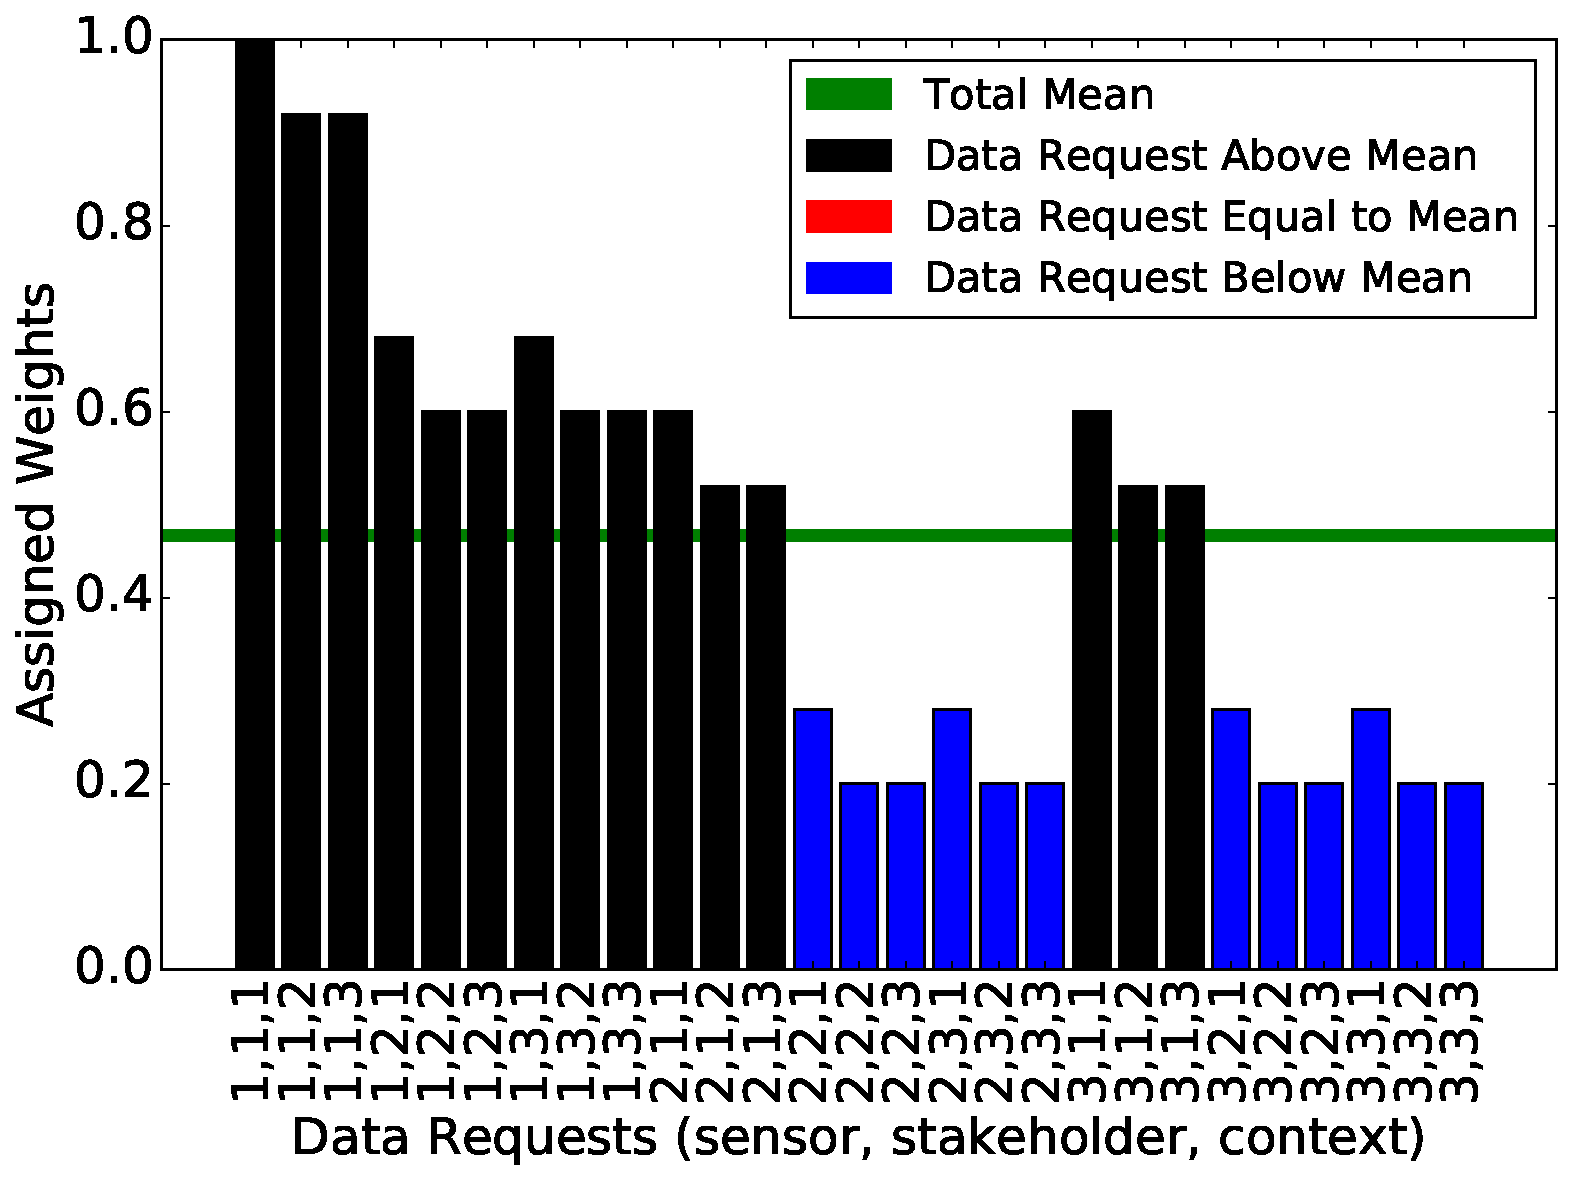
\includegraphics[width=0.5\linewidth]{./images/weight_4}}%
%  \subtop[Values of the Cost Matrix \label{cost4}]{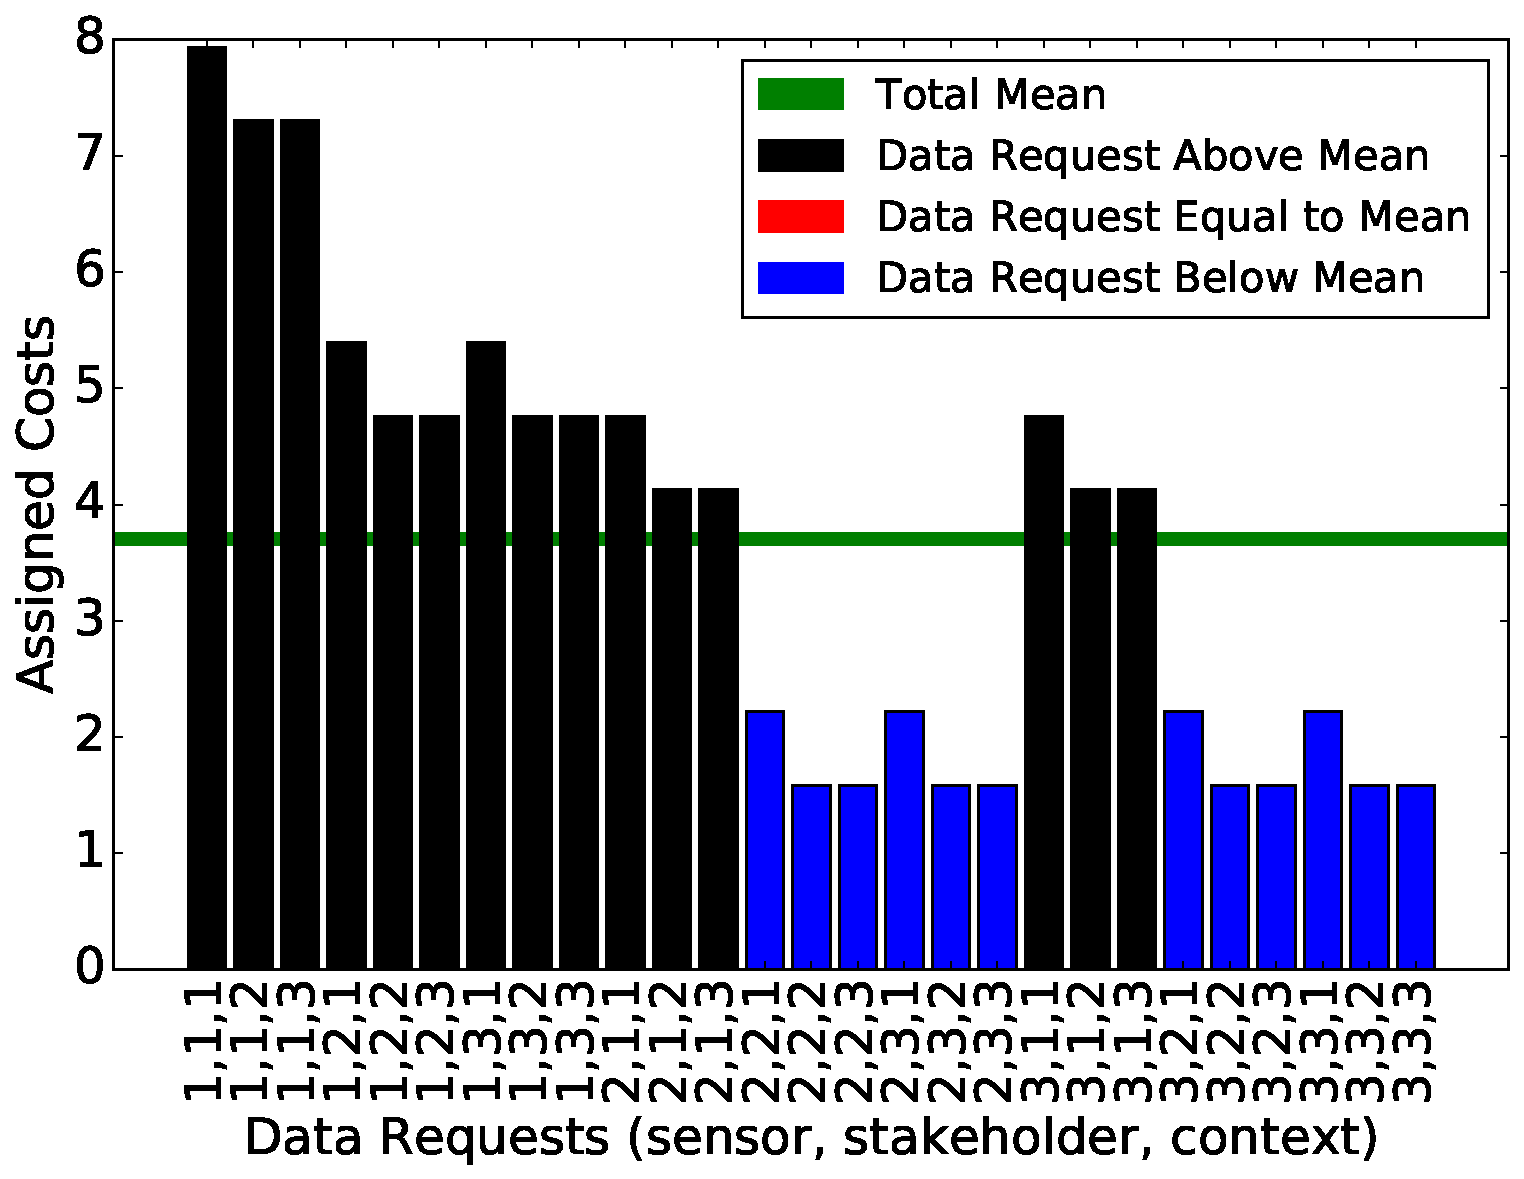
\includegraphics[width=0.5\linewidth]{./images/cost_4}}%
%  \caption{Examining Scenario 3}
%  \label{fig:scenatio4}
%\end{figure}


%\begin{figure}[ht!]
%\centering
%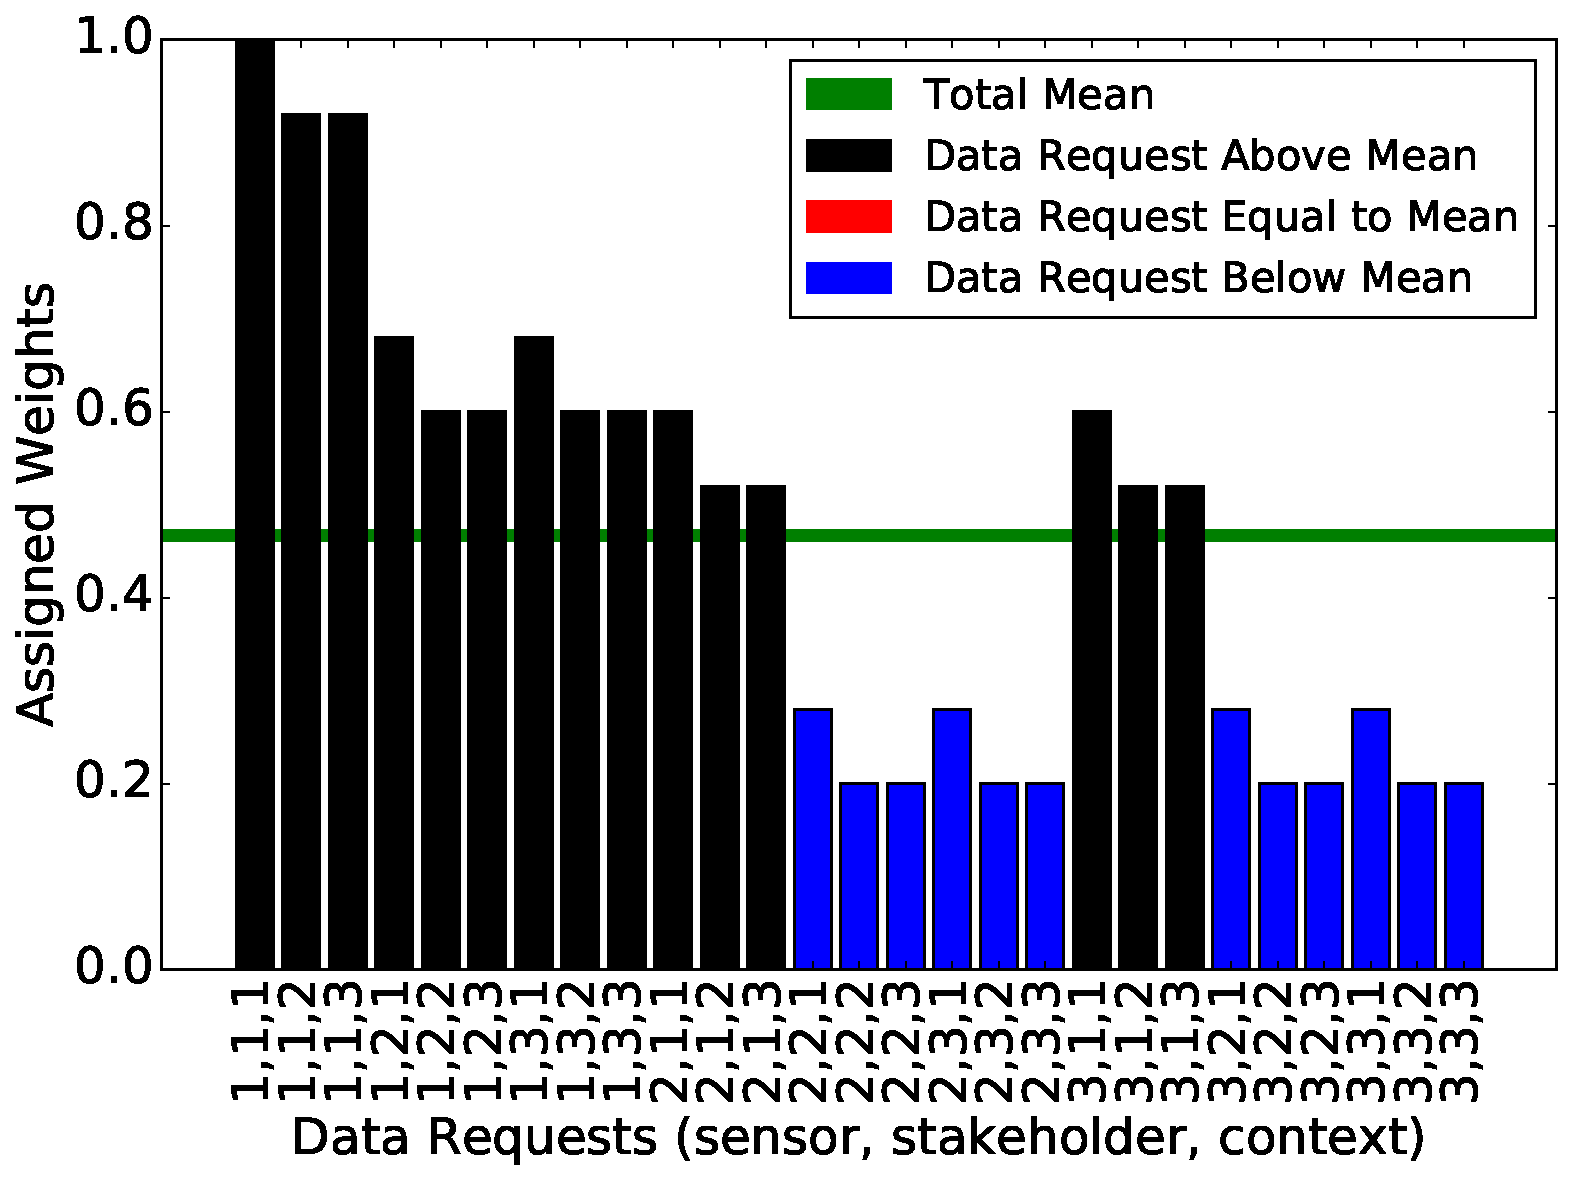
\includegraphics[width=\textwidth,keepaspectratio]{./images/weight_4}
%\caption{Values of the Weight Matrix\label{weight4}}
%\end{figure}
%
%\begin{figure}[ht!]
%\centering
%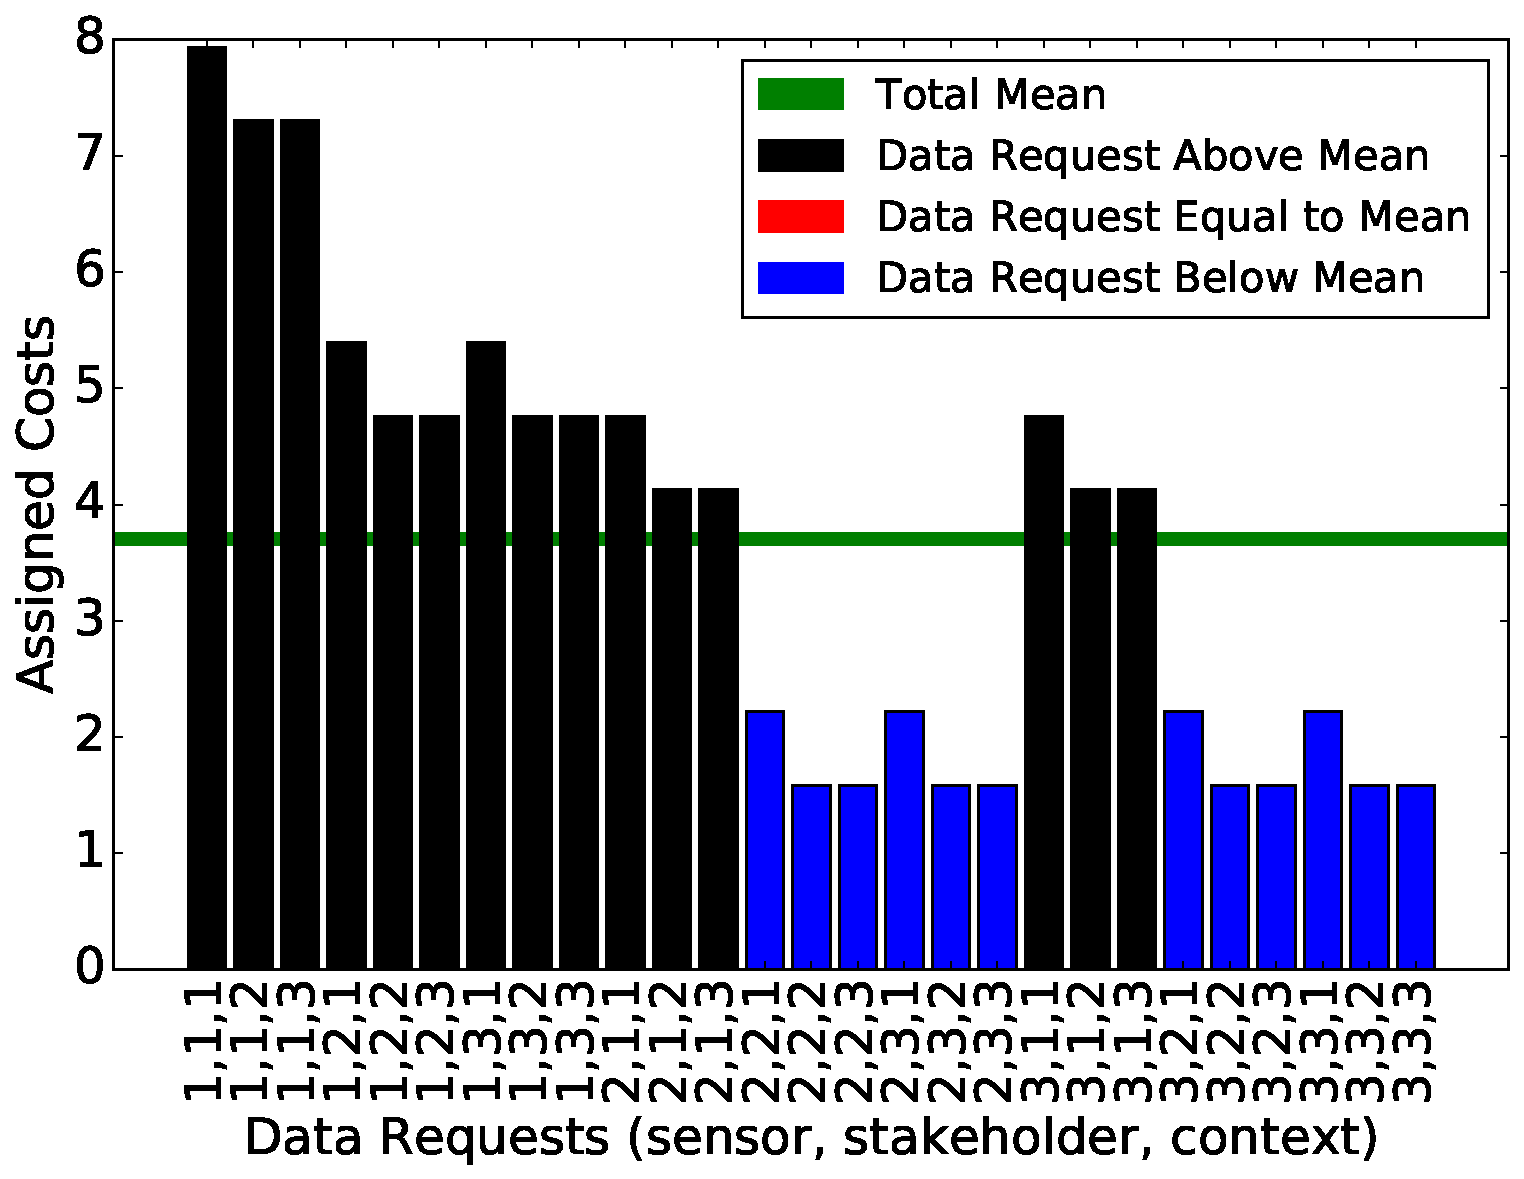
\includegraphics[width=\textwidth,keepaspectratio]{./images/cost_4}
%\caption{Values of the Cost Matrix \label{cost4}}
%\end{figure}

%\begin{figure}[htp]
%
%\caption{Table Schemas}
%\label{fig:st3}
%\end{figure}

The green horizontal line in the graph indicates the mean value of the weights and rewards. In general due to sub-features categorized as 5, those data requests receive a higher weight and reward. In some cases, the data requests receive a lower weight such as tuple (2,2,1),
(2,3,1),(3,2,1) and (3,3,1) tough context sub-feature 1 has a category of 5. This is due to the fact that sensor and stakeholder feature have a higher category of 5 and 4 respectively than the context feature. Since their sub-features are assigned a lower privacy intrusion category than context sub-features, the weight of the data requests is lower. This shows that even if a sub-feature may be regarded as very intrusive, it's weight changing ability depends on the category of the feature it belongs to.

Additionally, that data requests with at least two sub-features 1 are all above average. This witnesses the property of the model, which puts more emphasis on the perception of the features than the sub-features themselves. As seen in the figure, all the features with higher intrusion categorizations have weights and rewards that are well above average.

It can be concluded that the model assigns weights to data requests, by emphasizing on the feature's weights. A feature with a high category
has the ability to assign higher rewards with a highly categorized sub-feature. It also has the ability to lower the weight of a data request with a sub-feature l that is categorized lower. Features with lower categories contribute lesser to weight assignments, irrespective of their sub-feature categories.







